\documentclass[a4paper,12pt,oneside]{article}

\usepackage[
    top=0.6in,      % Reduce the top margin
    bottom=1in, % Keep bottom margin
    left=1in,   % Keep left margin
    right=1in,  % Keep right margin
    headheight=14pt,
    headsep=0.3in % Space between header and text
]{geometry}
\usepackage{graphicx}
\usepackage{amsmath, amssymb}
\usepackage{hyperref}
\usepackage{tikz}
\usetikzlibrary{shapes.geometric, arrows}
\usepackage{afterpage}
\usepackage{etoolbox}
\raggedbottom


\title{COP290: Spreadsheet Program Report}
\author{Team Members: \textbf{Nimit Jain, Shreyash Mohanty, Kunal Bisht}} 
\date{Semester 2024-2025, Sem II}

\begin{document}

\maketitle

\section{Introduction}
This report documents our spreadsheet program's design, implementation, and testing developed for COP290 . The program provides a command-line interface for managing a cell grid that stores integer values or formulas, supporting automatic recalculations and various commands.

\section{Design and Implementation}

\subsection{Key features }

\begin{itemize}
    \item Supports integer values and formulas.
    \item Automatic recalculations based on dependencies.
    \item Command-line navigation for large sheets.
    \item Built-in error handling for invalid inputs, division by zero, and circular dependencies.
    \item Enable/turn off output feature for batch processing.
\end{itemize}

\subsection{Overall Structure}
The project is structured into multiple modules, each handling different aspects of the spreadsheet. The key files and their purposes are:

\begin{itemize}
    
    \item \textbf{Node.c, Node.h}: Defines a structure ``Node''
 which stores the basic information about each cell of the spreadsheet.
    \item \textbf{Sheet.c, Sheet.h}: Defines a structure ``Sheet'' that stores the information about the spreadsheet and contains a matrix of node structures that constitute the spreadsheet.
    \item \textbf{parsing.c, parsing.h}: Handles user input parsing and assigns the properties of each of the nodes.
    \item \textbf{display.c, display.h}: Controls the spreadsheet display and handles the scroll functionalities.
    \item \textbf{validity.c, validity.h}: Ensures input validation and error handling.
    \item \textbf{Functions.c, Functions.c}: Implements all the basic functions. It also handles the functionality to check for cyclic dependencies and the addition and removal of edges in the graph during assignment or reassignment.
\end{itemize}

% \subsection{Node Structure}

% The core data structure used in the spreadsheet for representing cells and dependencies is the \texttt{Node} structure.

% \noindent The fields of the structure are described below:

% \begin{itemize}
%     \item \textbf{isValid}: Indicates whether the Node will be displayed as ERR or not. A node is shown as ERR iff it has a division by zero error or depends on a node with division by zero error.
%     \item \textbf{val}: Stores the numerical value of the Node.
%     \item \textbf{id}: Unique identifier for the node. For a node in the \(i\)th row and \(j\)th column, this identifier is defined as \( i \times (\text{number of columns}) + j \).
%     \item \textbf{OutNeighbours}: Pointer to a linked list storing nodes that depend on the Node.
%     \item \textbf{type}: Represents the type of the Node (e.g., constant, formula, etc.). Each function is assigned to a unique type. By default, the type is initialized to 0 which represents constant assignment.
%     \item \textbf{cell1, cell2}: Store references to other cells if the Node represents a formula or an arithmetic expression. They are set to -1 by default.
%     \item \textbf{op\_val}: Stores the numeric value in case of commands like cell=value+cell.
%     \item \textbf{operator}: Stores the mathematical operator used the in case of an arithmetic expression. 
% \end{itemize}
\section{Program Flow}
The execution flow of the spreadsheet program is organized into several key steps:

\begin{enumerate}
    \item \textbf{Input Reception:}  
    The main file begins by taking input from the user. This input can be either a command related to scrolling or enabling/disabling output, or it may be a cell assignment command.

    \item \textbf{Command Type Determination:}  
    The program first checks if the input corresponds to a scroll command or an enable/disable output command.  
    \begin{itemize}
        \item \textbf{Scroll/Output Command:} If the input is of this type, the main file calls the corresponding command from the display module. After executing the command, the program exits.
        \item \textbf{Cell Assignment Command:} If the input is not a scroll or output command, it is treated as a cell assignment, and the main file calls the \texttt{assign cell} function defined in the parsing module.
    %     \textbf{Example:} For an input such as \texttt{A1=MAX(A2:C2)}, the following properties are extracted:
    % \begin{itemize}
    %     \item \textbf{type:} 3 (corresponding to the \texttt{MAX} function)
    %     \item \textbf{isValid:} 1 (indicating a valid input by default)
    %     \item \textbf{cell1:} Hash value of \texttt{A2}
    %     \item \textbf{cell2:} Hash value of \texttt{C2}
    %     \item \textbf{op\_val:} 0
    %     \item \textbf{operator:} `\texttt{\textbackslash0}' (indicating no operator)
    % \end{itemize}
    \end{itemize}

    \item \textbf{Input Validation within \texttt{assign cell}:}  
    Once the cell assignment command is received, the \texttt{assign cell} function first validates the input using functions from the validity module.
    \begin{itemize}
        \item If the input is invalid, the \texttt{assign cell} function exits immediately, and the main function calls the display sheet function while also displaying an error.
        \item If the input is valid, the new properties are temporarily stored in variables for further processing.
    \end{itemize}

    \item \textbf{Cycle Detection and Topological Sorting:}  
    The temporarily stored properties are then passed to the \texttt{check cycle} function (from the functions module), which:
    \begin{itemize}
        \item Checks for cyclic dependencies within the spreadsheet.
        \item Simultaneously performs a topological sort on the directed acyclic graph (DAG) rooted at the cell whose value is being assigned.
    \end{itemize}
    \begin{itemize}
        \item If a cycle is detected, the \texttt{assign cell} function exits, and the main function subsequently calls the display sheet function while showing an error.
        \item If no cycle is found, the process continues.
    \end{itemize}
    The \texttt{check cycle} function is based on the observation that there is a cycle if and only if, in the new formula, there exists an incoming edge from one of the nodes already present in the computed topological order. If such an edge is found, it implies a cycle; otherwise, the process continues.


    \item \textbf{Updating Dependencies and Recalculation:}  
    For valid input with no detected cycles:
    \begin{itemize}
        \item The \texttt{delete\_edge} function is called to remove all outdated dependencies associated with the cell.
        \item The cell’s properties are then updated with the new values stored in the temporary variables.
        \item The \texttt{add\_edge} function is invoked to add new dependencies based on the updated cell.
        \item Finally, the \texttt{recalculate node} function is called to recompute all affected cells in the subgraph, following the topological order.
    \end{itemize}

    \item \textbf{Display Update:}  
    After the cell assignment process is complete, control returns to the main function, which then calls the display sheet function to present the updated state of the spreadsheet.
\end{enumerate}
\section{Test Suite}
The test suite for this project is implemented in C and is integrated into the build process. It covers:
\begin{itemize}
    \item Basic cell assignments and arithmetic operations.
    \item Input validation and error handling.
    \item Dependency tracking and recalculation of cells.
    \item Edge cases such as division by zero and circular dependencies.
\end{itemize}
To run the test suite, execute:
\begin{verbatim}
make test
\end{verbatim}
The suite automatically compares program output against expected results, ensuring the correctness of all functionalities.

\section{Challenges}
Several challenges were encountered during the development of this spreadsheet program:
\begin{itemize}
    \item \textbf{Dependency Tracking:} Efficiently managing and updating the dependencies among cells to trigger only the necessary recalculations.
    \item \textbf{Circular Dependency Detection:} Implementing a robust and efficient mechanism to detect cycles in formulas, ensuring that the program correctly finds the topological ordering of the graph and simultaneously detects cycles.
    \item \textbf{Node Structure Design:} Designing the structure of the node and deciding what information is required during recalculations and cycle checks.
    \item \textbf{Robust Parsing:} Accurately parsing complex user inputs, including formulas and commands, while gracefully handling invalid or erroneous inputs.
\end{itemize}

\section{Demo Video and GitHub Repository}
For a demonstration of the program in action and access to the source code, please refer to the following links:
\begin{itemize}
    \item \textbf{Demo Video:} \url{https://your-demo-video-link.com}
    \item \textbf{GitHub Repository:} \url{https://github.com/Kunal-0510/COP290_C_Lab}
\end{itemize}

\vspace{-2.5em} % Pull diagram closer to previous text

\noindent\begin{figure}[h!]
\section{Flow Diagram for Computation of a Single Command}
\centering
\resizebox{\textwidth}{!}{ % Scale diagram horizontally
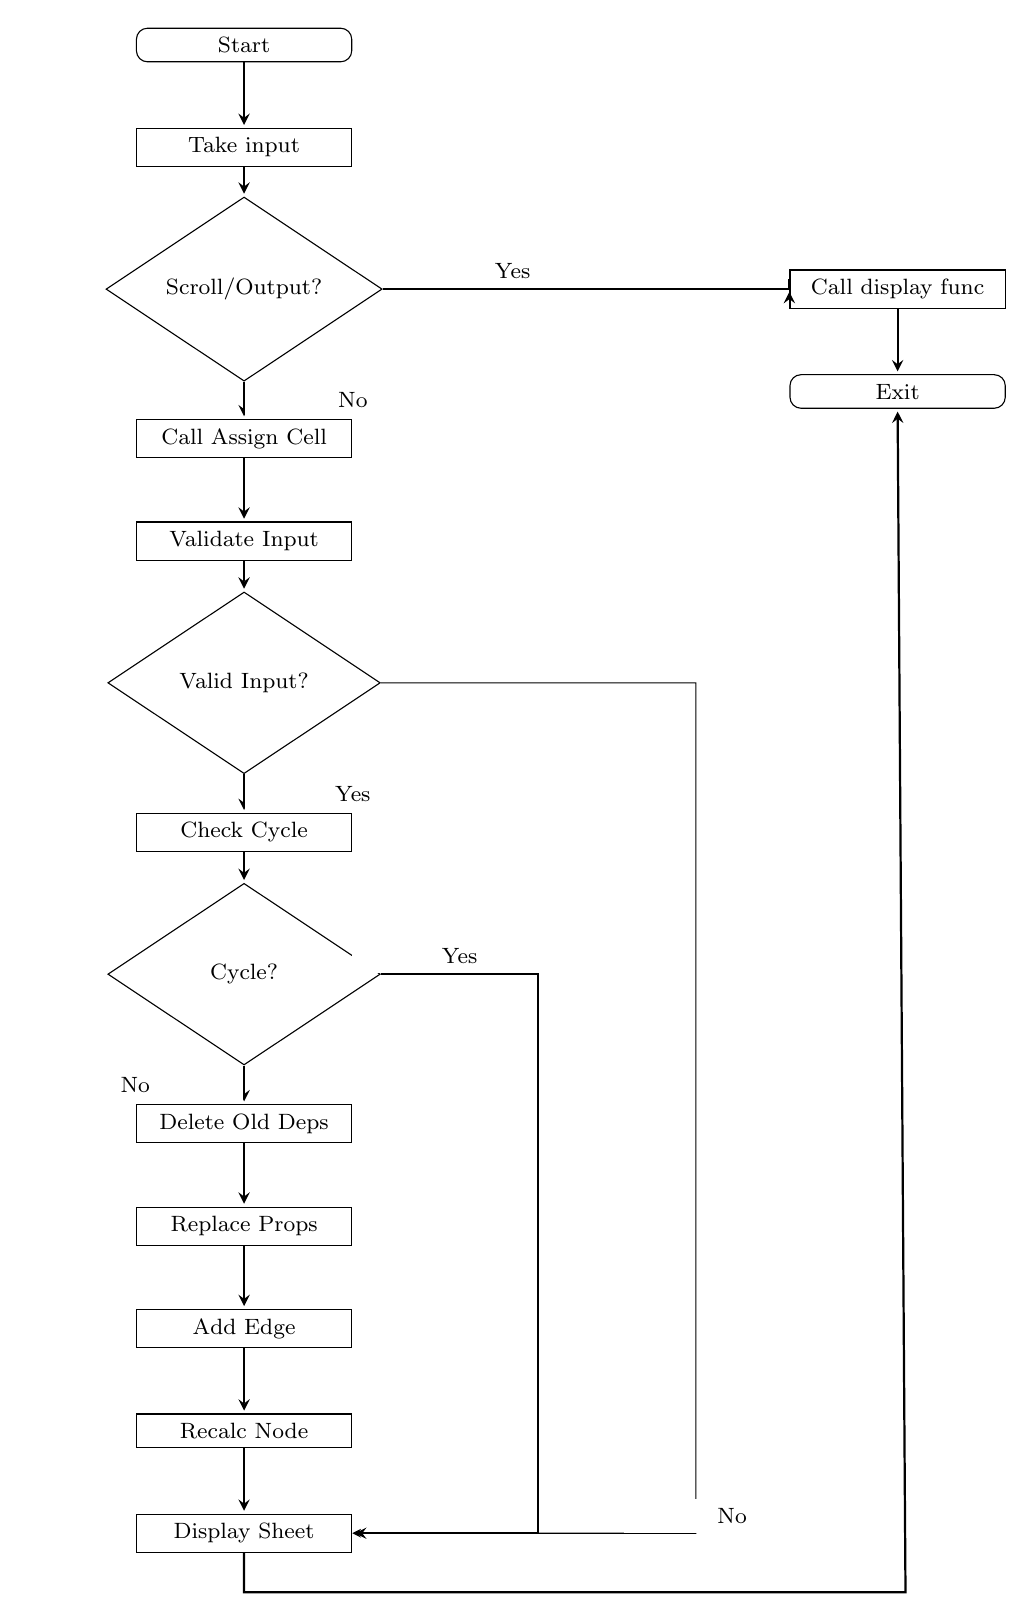
\begin{tikzpicture}[
    node distance=1.3cm,
    every node/.style={font=\footnotesize, fill=white, text centered, text width=2.5cm},
    >=stealth,
    arrow/.style={->, thick, shorten >=1pt},
    startstop/.style={rectangle, rounded corners, draw=black, minimum width=2.5cm},
    process/.style={rectangle, draw=black, minimum width=2.5cm},
    decision/.style={diamond, aspect=1.5, draw=black}
]
% Nodes
\node (start) [startstop] {Start};
\node (input) [process, below of=start] {Take input};
\node (checkCommand) [decision, below of=input, yshift=-0.5cm] {Scroll/Output?};
\node (executeCommand) [process, right of=checkCommand, xshift=7cm] {Call display func};
\node (exit) [startstop, below of=executeCommand] {Exit};
\node (assignCell) [process, below of=checkCommand, yshift=-0.6cm] {Call Assign Cell};
\node (validateInput) [process, below of=assignCell] {Validate Input};
\node (invalidInput) [decision, below of=validateInput, yshift=-0.5cm] {Valid Input?};
\node (checkCycle) [process, below of=invalidInput, yshift=-0.6cm] {Check Cycle};
\node (cycleFound) [decision, below of=checkCycle, yshift=-0.5cm] {Cycle?};
\node (deleteEdge) [process, below of=cycleFound, yshift=-0.6cm] {Delete Old Deps};
\node (replace) [process, below of=deleteEdge] {Replace Props};
\node (addEdge) [process, below of=replace] {Add Edge};
\node (recalc) [process, below of=addEdge] {Recalc Node};

\node (display) [process, below of=recalc] {Display Sheet};

% Arrows
\draw [arrow] (start) -- (input);
\draw [arrow] (input) -- (checkCommand);
\draw [arrow] (checkCommand.east) -| (executeCommand.west) node[pos=0.7, above, xshift=-100pt]{Yes};
\draw [arrow] (executeCommand) -- (exit);
\draw [arrow] (checkCommand.south) -- (assignCell.north) node[midway, right]{No};
\draw [arrow] (assignCell) -- (validateInput);
\draw [arrow] (validateInput) -- (invalidInput);
% "Valid Input?" decision: "Yes" branch goes directly to Check Cycle
\draw [arrow] (invalidInput.south) -- (checkCycle.north) node[midway, right]{Yes};
% "Valid Input?" decision: "No" branch goes directly to Display Sheet with a ]-shaped arrow
\draw [->] (invalidInput.east) 
            -- ++(4cm ,0) 
            -- ++(0,-10.8cm)
            
            
            -- (display.east)node[pos=0.7, above, xshift=100pt]{No};
\draw [arrow] (checkCycle) -- (cycleFound);
% "Cycle?" decision: "Yes" branch goes directly to Display Sheet with a ]-shaped arrow
\draw [arrow] (cycleFound.east) 
            -- ++(2cm,0)node[midway, above]{Yes}
            |- (display.east) ;
% "Cycle?" decision: "No" branch goes to Delete Old Deps
\draw [arrow] (cycleFound.south) -- (deleteEdge.north) node[midway, left]{No};
\draw [arrow] (deleteEdge) -- (replace);
\draw [arrow] (replace) -- (addEdge);
\draw [arrow] (addEdge) -- (recalc);
\draw [arrow] (recalc) -- (display);

% L-shaped arrow from Display Sheet to Exit
\draw [arrow] (display.south) 
            -- ++(0,-0.5cm)
            -- ++(8.4cm ,0)
            
            --(exit.south);
\end{tikzpicture}
}
\end{figure}
% \vspace{-3em} % Compensate after diagram




\end{document}
